%\todomacaluso{
%	\begin{itemize}
%		\item General description of the framework
%		\item Discussion about the motivation and the importance of this framework, such as the necessity of a Reinforcement Learning Framework to test different algorithms with different environments providing the same interface.
%		\item One contribution of the thesis: the creation and design of an OpenAI Gym environment for Anki Cozmo Environment with connection to chapter 4.
%	\end{itemize}	
%}

\chapter{Tools and Frameworks} \label{ch:ch3}

This chapter aims to describe the main tools and frameworks used to develop the project of this thesis. The first section will describe OpenAI Gym framework, a central toolkit for developing and comparing reinforcement learning algorithms, and explain why this tool is essential for reinforcement learning research.
The second part of this chapter will outline Cozmo, the powerful toy robot developed by Anki that we used as an agent in the reinforcement learning scenario to apply algorithms to try solving autonomous self-driving tasks: \vref{ch:ch5} will report the analysis and description of these experiments. This section will also report a set of available alternatives to Cozmo, explaining the motivations underlying the final choice.
The description about PyTorch, an optimised tensor library for deep learning using GPUs and CPUs used to build up the convolutional neural network of this work, and the related comparison with TensorFlow will occupy the last part of this chapter.

\section{OpenAI Gym}

Nowadays, OpenAI Gym, released in 2016 with its public beta, is one of the most popular toolkits and frameworks in the reinforcement learning scenario. A brief analysis of reinforcement learning research could be useful to outline the motivations underlying the need for a reinforcement learning framework.

As reported previously in  \vref{ch:ch2}, reinforcement learning is a subfield of machine learning dedicated to the world of decision making and motor control: researchers study how an agent can learn and improve to achieve a specific goal in a complex, usually unknown environment. This machine learning paradigm is becoming more and more attractive for both researchers and industries because of its visionary property of being very general. A reinforcement learning algorithm can be exploited to control a robot's motor in order to make it capable of running or jumping, play a videogame or a board game, make critical business decisions like pricing and inventory management, but also learn how to invest in financial trading environments. The generality of reinforcement learning became engaging thanks to the remarkable results achieved in many challenging environments, as reported previously in \vref{ch:ch2}.

Despite these appealing features, the research was slowed down by other circumstances, no less critical.
The need for better benchmarks represents the first factor. As an example, the abundant availability of conspicuous datasets like \textit{ImageNet} \cite{deng2009imagenet} has driven supervised learning improvement in the research. For what concerns reinforcement learning, the nearest equivalent to supervised learning datasets would be a broad collection of different environments in order to test various algorithms with different kinds of observations or rewards.
The second withdraw of this approach to learning is the lack of standardisation of environments designed in publications. In reinforcement learning, subtle differences in problem definition, reward function design or action space typology could make the difficulty of the task grow.  This fact threatens to slow down and corrupts experiments reproducibility making an objective comparison between the results of different papers almost impossible.

The need to fix both problems was the primary motivation behind the design and implementation of OpenAI Gym.

\subsection{Environments}

The agent and the environment represent the main components of reinforcement learning. The choice of OpenAI was to implement and provide the abstraction mainly for environments, not for agents. They decide to provide a standard environment interface instead of forcing the developer to use pre-defined agent interfaces: the motivation behind this choice was to leave developers independent in the design of the agent, the core of reinforcement learning, and facilitate the creation and usage of environments. Thanks to this approach, all agents implemented with OpenAI Gym can be used with the whole set of environments provided by the framework. Therefore, it is possible to create a personalised environment to suit the needs of a specific experiment that can be used by all agents exploiting OpenAI Gym environment interfaces.

In this scenario, we realised the first contribution to our thesis. Thanks to this framework features, we implemented an OpenAI Gym environment capable of interacting with Anki Cozmo by providing a binding between functions of Cozmo SDK and interfaces of the reinforcement learning framework. In \vref{ch:ch4} we will provide further information and details about our contribution.

The importance related to the high quantity of environment is fundamental to build a reliable and sustainable framework for reinforcement learning algorithms. For this reason, OpenAI Gym contains a various and heterogeneous environment database, ready to be used.

\subsubsection{Interface Functions}

Exploring OpenAI Gym, it is essential to focus on the most crucial interface functions that the agent will exploit to interact with the environment.
The functions which constitute the skeleton of an OpenAI Gym environment are the following:
\begin{itemize}
	\item \texttt{def step(self, action)}: through this function, the agent can communicate the action it wants to take. The input data depends on the type and number of variables in the actions space (e.g.\ discrete or continuous). As will be discussed in \vref{subsec:observations}, the values returned by this function represent the environment state after the manipulation caused by the agent action. Thanks to these data, the agent will be able to select the next action following the reinforcement learning loop.
	\item \texttt{def reset(self)}: during the episode, internal variables of the environment changes, influenced by the action taken previously. This function allows the agent to restart the initial situation of the environment. This procedure is particularly helpful when an episode finishes and the agent has to restart the next learning episode in a brand new copy of the environment.
	\item \texttt{def render(self, mode='human', close=False)}: this function is mainly used in simulated environments. It enables the visual render (if available) of the environment.
	\item \texttt{def close(self)}: the final function to close the environment after the end of all experiments and episodes.
\end{itemize}

\subsubsection{Available environments}

To date, OpenAI Gym includes the following environments:
\begin{itemize}
	\item \textbf{Algorithms}: learning to imitate computations, such as copying or reversing symbols from the input tape, is the main aim of this typology. These environments might seem easy to be solved by a computer, but it is important to remember that the objective here is to learn to solve these tasks purely from examples. Therefore, it is possible to vary the sequence length to increase or decrease task difficulties easily.
	\item \textbf{Atari}: \textit{Atari 2600} is a home video game console developed in 1977 which spread the use of general-purpose CPUs into gaming with game code distributed through cartridges. This environment section provides a database which contains more than 100 environments emulating Atari 2600 videogames. OpenAI Gym exploits \textit{Arcade Learning Environment (ALE)} \cite{bellemare2013arcade} providing RAW pixel images or RAM as observation of the environment.
	\item \textbf{Box2D}: in this group is possible to find some continuous control tasks in a simple 2D simulator such as \textit{BipedalWalker}, \textit{CarRacing} and \textit{LunarLander}
	\item \textbf{Classic Control}: this class provides a set of problem borrowed by control theory and widely exploited in the classic reinforcement learning literature. Some task examples are balancing a pole on a cart or swing up a pendulum.
	\item \textbf{MuJoCo}: this collection contains continuous control tasks running in a fast physics three-dimensional simulator called \textit{MuJoCo} which stands for \textit{Multi-Joint dynamics with Contact}. This physics engine aims to facilitate research and development in robotics, biomechanics, graphics and animation. The simulator is particularly suitable for model-based optimisation allowing to scale up computationally-intensive techniques.
	      Thanks to its features, it became useful as a source for reinforcement learning algorithms. \cite{todorov2012mujoco}
	\item \textbf{Robotics}: OpenAI released this algorithm typology to provide eight robotics environments with manipulation tasks significantly more difficult than the MoJoCo ones. It contains \textit{Fetch}, a robotic arm to move and grab objects, and \textit{ShadowHand}, a robotic hand to manipulate and grab pens, cubes and balls. \cite{ingredientsRoboticsResearch}
\end{itemize}

\subsection{Observations} \label{subsec:observations}

As previously reported, the \texttt{step(self, action)} environment interface is the most important one because it contains the behaviour definition of the environment that reacts to agent actions.
Indeed, the agent has to know in which way its actions are influencing the environment in order to stop doing random actions and start making valuable decisions.

In order to provide this type of information to the agents, the \texttt{step} function returns four relevant values that reinforcement learning algorithms can exploit to determine the best action to do in the future.
These values are:
\begin{itemize}
	\item \textbf{\texttt{observation (object)}}: a specific object which represents the environment observation and shows the changes provoked by agent actions. Its structure and interpretation depend on the implementation of the specific environment. For example, it could represent the raw pixel data from a camera, the status of a board game or physics data of a robot (joint angles and velocities).
	\item \textbf{\texttt{reward (float)}}: this is the fuel of the reinforcement learning algorithms. This value represents the reward achieved thanks to the action taken by the agent. The reward for each action can change among environments, but this is the crucial information to enable the agent to learn.
	\item \textbf{\texttt{done (boolean)}}: this value is a simple boolean that signals the agent when the episode ended and it is time to reset the environment to start a brand new episode.
	\item \textbf{\texttt{info (dict)}}: a Python dictionary to monitor and show diagnostic information useful for debugging. The agent could use it as additional information in the learning process, but the documentation of OpenAI Gym does not recommend to use this data in the learning process to maintain the coherence with the reinforcement learning loop.
\end{itemize}

The last important thing to report about OpenAI Gym framework is the definition of \texttt{Spaces}. As reported in the second chapter, an environment consists of the action space and the observation space. Both can provide discrete or continuous values: this distinction is fundamental to determine the usage of a specific algorithm rather than others to solve a given task better. For this reason, OpenAI Gym provides \texttt{Discrete} and \texttt{Box} to initialise discrete and continuous spaces, respectively. It allows the user to define a lot of features useful in the learning process, such as a maximum and minimum value setup or a default function to instantly sample a random value from the defined space.

\section{Anki Cozmo}

\begin{figure}

	\begin{minipage}[t]{0.48\linewidth}
		\centering
		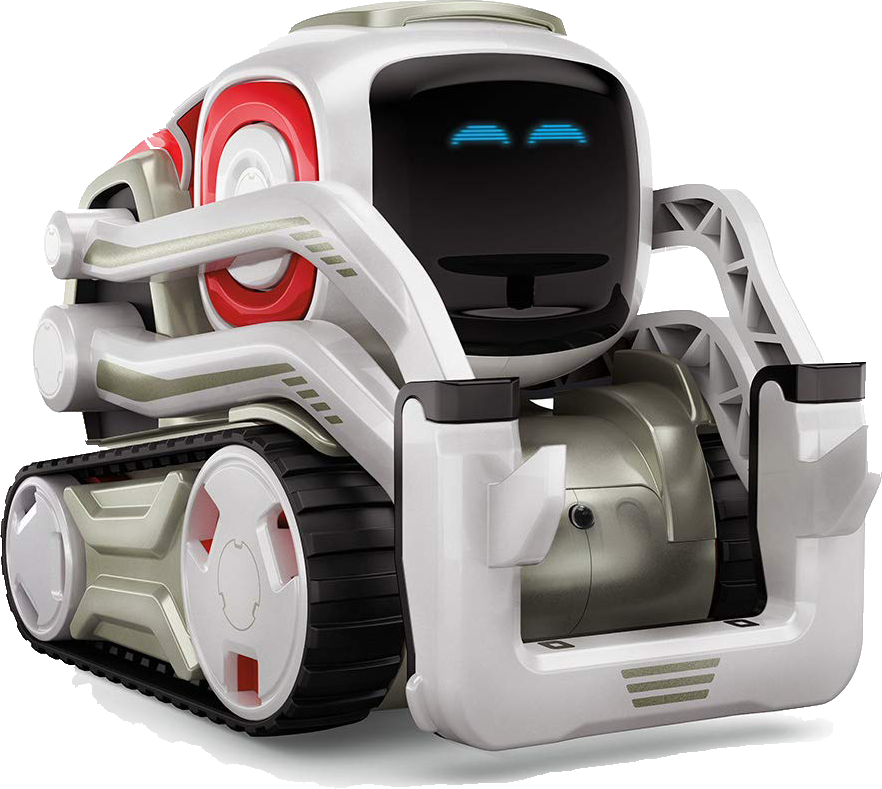
\includegraphics[height=0.25\paperwidth]{img/cozmo_inside_1.png}
	\end{minipage}
	\begin{minipage}[t]{0.48\linewidth}
		\centering
		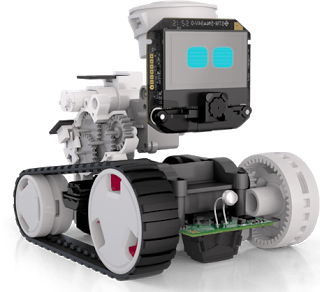
\includegraphics[height=0.25\paperwidth]{img/cozmo_inside_2.png}
	\end{minipage}

	\caption[Anki Cozmo Robot]{On the left there is a photo of Anki Cozmo in action, while on the right side there is a graphical reconstruction of the whole set of gears and hardware inside the robot.}
	\label{fig:cozmo_inside}
\end{figure}

Especially in the latest decades, human beings have started a complicated relationship with robots. They are very fascinated by the prospect of artificial intelligence offered by recent researches and applications. However, they are apprehensive and worried at the same time because of the apocalyptic plot that many sci-fi films show and the big promise of automation, capable of replacing human workers in the future.
However, all these concerns disappear after meeting Cozmo, the palm-sized toy robot developed by the San Francisco-based company Anki and available on the market since 2016.
On first glance, Cozmo might appear as one of the cutest toy robots: not surprisingly Anki employed the guidance of Carlos Baena, the former Pixar animator, to design this robot.
Therefore, it can interact with people using a small display screen together with audio effects to mimic human emotional reactions and responses.
The result is a toy robot WALL-E-inspired both aesthetically and personality-wise, powered up by artificial intelligence to move and discover the surrounding environment. Thanks to the built-in camera, Cozmo can remember faces and recite names, but also to plan paths and play various games with its three cubes that carry sensors and lighting.

Despite these entertaining, but not so technical facts, Cozmo hides a lot of powerful features under the hood. Anki developers produced a high-quality Python SDK that allows developers to take control of the whole set of Cozmo sensors and actuators thanks to the interaction granularity offered by functions and interfaces.
This section aims to outline the hardware and software architecture hidden underneath the cute Cozmo bodyworks, together with a comparison with the alternatives available to design the reinforcement learning system of this thesis. An essential inspiration in the writing of this section came from \cite{mellon2017cognitive}, \cite{touretzky2018cozmopedia} and Anki Forums \footnote{Anki Cozmo SDK Forums: \href{https://forums.anki.com/}{https://forums.anki.com/}}.

\subsection{Cozmo Architecture}

It is possible to define Cozmo as a vision-guided mobile manipulator, one of the first consumer robot which can boast vision among its features. However, as reported before, the features it shows during the normal toy usage, do not equal the number of interfaces and functions made available to developers. The hardware and the software developed for Cozmo makes it the right choice to fast prototyping computer science projects: it is the main reason why we decided to exploit Anki Cozmo instead of other alternatives.
The SDK provided by Anki consists of a comprehensive set of low- and high-level functions which grants full access to sensor data providing the right flexibility, simplicity and granularity to satisfy every developer needs. It is versatile because it could be easily connected with hundreds of third-party libraries to augment Cozmo capabilities. Therefore, it is an entirely open-source SDK to give the community the freedom to customise and contribute.

\Vref{fig:cozmotear1,fig:cozmotear2} shows technologies, the hardware and software involved in the production of Cozmo. The first image represents stacks and connections between the robot core and the mobile application provided by Anki, while the second one shows the interaction between the last-mentioned application and the Python user program on the development machine. The reader can retrieve a global perspective about the whole Cozmo architecture by merging these two figures.

\begin{figure}
	\centering
	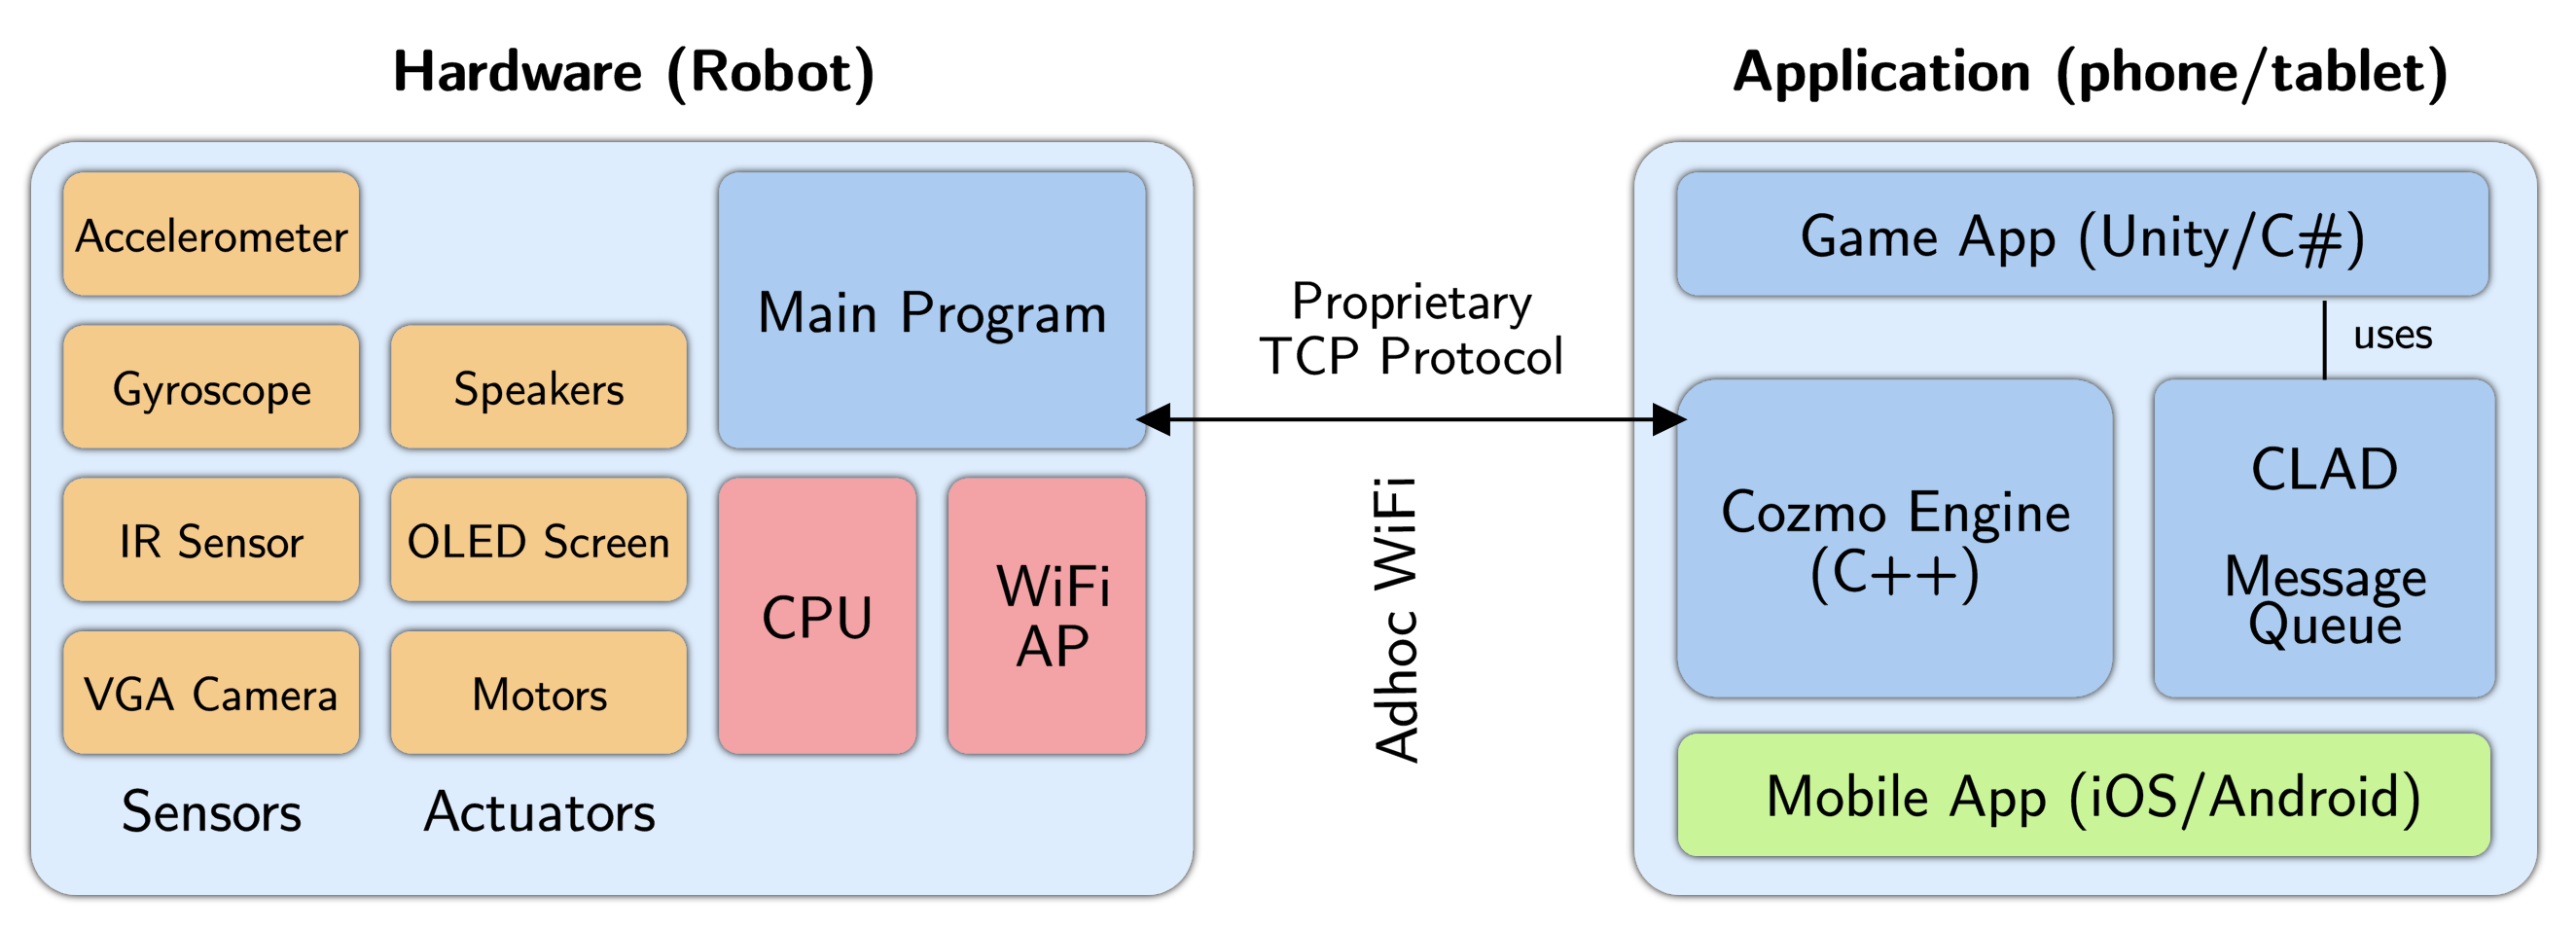
\includegraphics[width=\textwidth]{img/cozmo-hw.png}
	\caption[Interaction Robot/Application]{Interaction between the Robot and the mobile application stack. The robot main program interacts with the Cozmo Engine (C++) implemented in the mobile application through a proprietary TCP protocol established using and ad-hoc WiFi connection. \cite{mellon2017cognitive}}
	\label{fig:cozmotear1}
\end{figure}

Starting from \vref{fig:cozmotear1}, it is noticeable that Cozmo has a lot of sensors and actuators, which enable it to move and understand the surrounding environment. For what concerns the sensor part, the VGA Camera is the crucial component exploited in the thesis. This camera provides a grayscale image with 320$\times$240. Anki reported a camera resolution equal to 640$\times$480, but the latest firmware version supports only the lower resolution. Furthermore, the camera can detect and acquire colours, but the firmware limits this feature to maintain the bandwidth stable and avoid overloads or slowdowns in the communication with the mobile application and subsequently, the user program running on the computer.
The camera has approximately 60° field of view (FOV) and 290mm focal length.

As regards the actuators column, Cozmo can explore the world thanks to its four motors and over fifty gears. Instead of having wheels, this robot has two tracks to navigate: it can steer and move freely by controlling the speed of each track.
Another moving part is the head that can move up or down to direct the camera and the display. It also has a forklift with which it can lift objects or the cubes available in the kit.

Cozmo can perform one single action at a time: if the current action is not yet complete and the request of a new action occurs, the new action fails with a \textit{tracks locked} failure code. For this reason, the SDK does not allow the execution of multiple actions. Despite this fact, it is easy to notice that Cozmo animations and behaviours typically use combinations of actions: indeed the user can send simultaneous actions to the robot by calling them using \texttt{in\_parallel=True} in its script, but these actions have to belong to a different action track. This approach allows the parallel execution of actions, provided that they use different tracks.
Cozmo software architecture holds seven independent action tracks:

\begin{itemize}
	\item \textbf{HEAD}: raise/lower robot head.
	\item \textbf{LIFT}: raise/lower robot forklift.
	\item \textbf{BODY}: wheels or treads actions for driving and turning.
	\item \textbf{FACE\_IMAGE}: actions with the OLED display such as animations or faces.
	\item \textbf{EVENT}: for this action type Anki does not release further information.
	\item \textbf{BACKPACK\_LIGHTS}: actions or animations of lights on Cozmo back.
	\item \textbf{AUDIO}: speech or sound effects emitted by the robot.
\end{itemize}

The project of this thesis mainly exploited the body action track to move the robot in the environment: it also employed head and lift tracks, but only to position the robot head to provide images about the track to the main program and the reinforcement learning agent. The usage of parallel operations was not necessary.

The Cozmo hardware includes an onboard CPU and a WiFi access point, thanks to which the user can interact with the robot. However, to activate this communication, it is necessary to install the Cozmo Android/iOS application on a personal tablet or smartphone. This application is the same used to play with the toy-side of Cozmo, but in its settings, there is a function to enable Cozmo development mode.
After connecting the chosen personal device to the robot through a simple WiFi connection, the application manages to create a proprietary TCP protocol to interact directly with the main robot program.
The creators of Cozmo developed this mobile application using C++ to implement the \textit{Cozmo Engine}, the component which shall be responsible for the TCP communication with the robot. To design and implement the game experience and the graphical user interface, they used Unity and C\#.

This last-mentioned part utilises the component internally designed and implemented by Anki to provide a contact point between the Cozmo SDK installed in the development machine, as shown in \vref{fig:cozmotear2}: the C-like Abstract Data language (CLAD).
The fundamental idea behind this tool is to make the process of serialisation, communication and deserialisation of data structures written in Python easier for the developer. In practice, for every data which has to pass over the wire, files with extension \texttt{.clad} to define enums, structures and messages are generated: their syntax is similar to C struct one. After that phase, this tool auto-generates Python, C++ and C\# code for each structure previously defined. This process allows the user to define a specific message in Python and to send it to the C++ engine where it will be deserialised automatically, avoiding problems and sources of bugs coming from intricate underlying details.

\begin{figure}
	\centering
	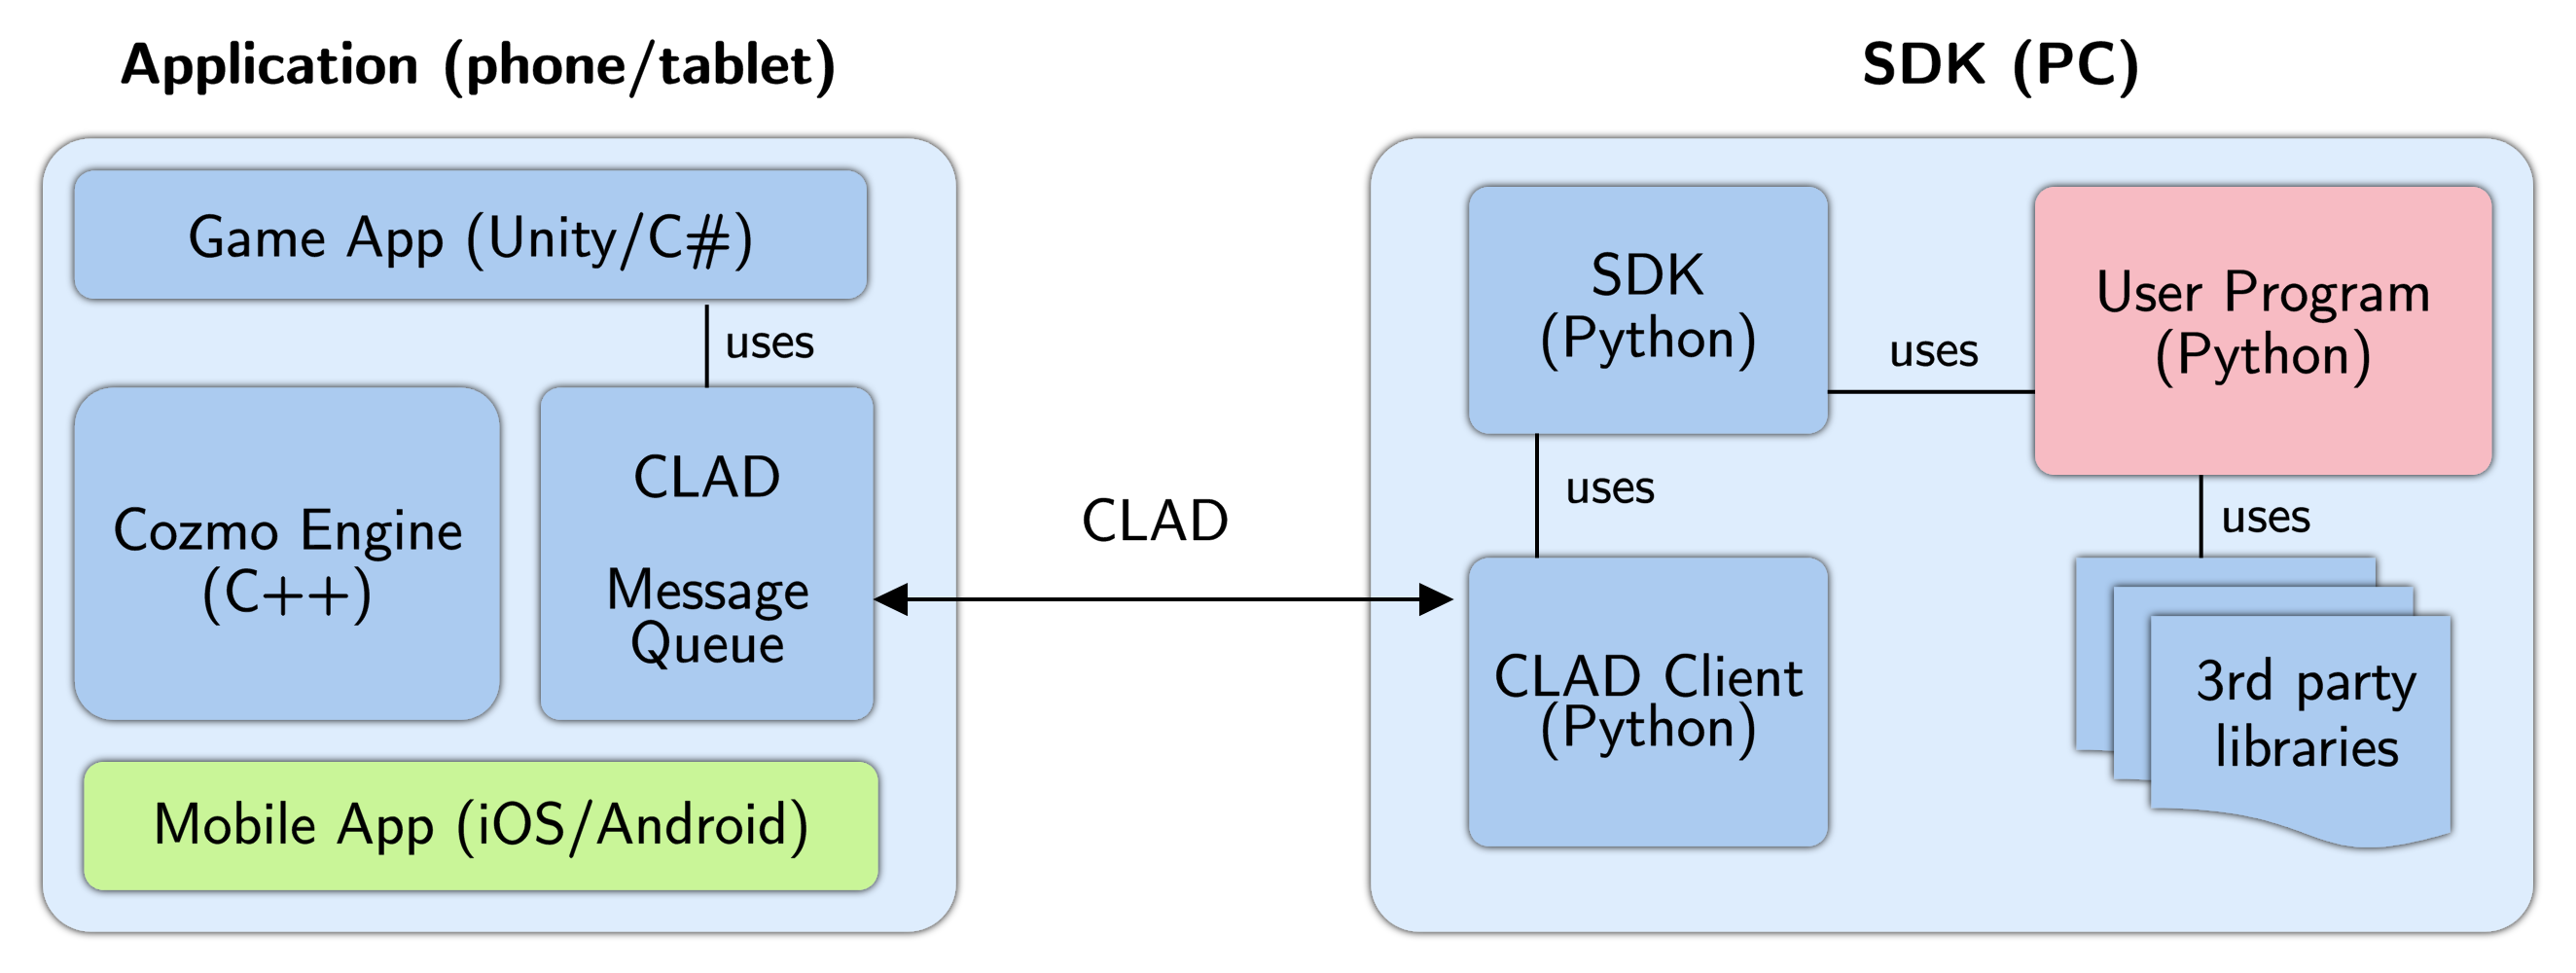
\includegraphics[width=\textwidth]{img/cozmo-sw.png}
	\caption[Interaction Application/PC]{Interaction between the mobile application stack and the Python user program. Anki designed a C-like Abstract Data Language (CLAD) to implement the connection between the Cozmo SDK and the Cozmo Engine on the mobile application. This approach puts a decoupling layer between Python interfaces and low-level functions to make prototyping easier and fast-forwarding for developers. \cite{mellon2017cognitive}}
	\label{fig:cozmotear2}
\end{figure}

This approach results in a process method much lighter than the one provided by \textit{Protocol Buffers (Protobuf)} by Google: even then, the main aim of this implementation choice was reducing the network bandwidth.
Taking all arguments into account, CLAD is the protocol used for the interaction between the SDK and the C++ Engine that allows the developer to not care about the low-level part of the code and to focus on the high-level logic using Python. It is also useful to maintain the same interface for the user even if low-level logic changes occur.

In this case, the CLAD communication messages exploit a wired connection between the mobile device and the computer with a simple USB cable. In this thesis, we used an Android tablet to run the experiments, and for this reason, we used the \textit{Android Debug Bridge (ADB)} to make this exchange possible.
It is a command-line tool included in the \textit{Android SDK Platform-Tools} package that allows the communication between the computer and Android devices. It facilitates many device actions such as installing, debugging apps or running a variety of commands on a device. It is a client-server program that consists of three components: it includes a \textit{client} hosted in the development machine, a \textit{daemon (adbd)} which runs the commands on the device as a background process and finally a \textit{server}, a background process in the development machine that manages the communication between the two previous components.

The last step to start programming with Cozmo SDK is to install it in a development machine following the instruction provided by its documentation \footnote{Cozmo SDK Documentation: \href{http://cozmosdk.anki.com/docs/index.html}{http://cozmosdk.anki.com/docs/}}.


\subsection{Why Cozmo?}

Before starting the development of this thesis project, we spent some time analysing the small car market situation in order to find out the right choice for our specific needs. In addition to Anki Cozmo, the ideal alternatives in the self-driving scenario when we started this thesis were \textit{AWS DeepRacer Vehicle} and a customised car implemented from scratch exploiting \textit{Donkey \textregistered
	Car library}.

This section part aims to briefly describe the main alternatives to Anki Cozmo listing strengths and weaknesses for each approach to motivate the final choice made.

\subsubsection{AWS DeepRacer}

\textit{AWS DeepRacer} is a platform developed by Amazon to learn and refine machine learning, reinforcement learning algorithms and techniques on AWS DeepRacer vehicle.

The whole ecosystem consists of two main part:
\begin{itemize}
	\item \textbf{AWS DeepRacer Car}. It is a 1/18 scale race car developed and built to test reinforcement learning algorithms on a real track. It aims to show how the reinforcement learning model trained in a simulated environment can be conveyed to the real-world by using cameras to view the track and the model to control throttle and steering. It has a lot of interesting specifications under the hood such as Intel Atom \textsuperscript{\textregistered} Processor, 4GB of RAM, an expandable 32GB of storage to accommodate the trained model and a 4-megapixel camera with MJPEG.
	\item \textbf{AWS DeepRacer Simulator}. The user can build his models in \textit{Amazon SageMaker} and train, test and iterate the learning process using the racing simulator. It offers an integrated environment hosted on the AWS cloud to experiment and optimise algorithms to apply to the autonomous driving model.
\end{itemize}

There are many advantages in using the DeepRacer stack. It offers an integrated approach where the developer has to focus just on reinforcement learning: indeed, it abstracts a significant part of the software giving the developer the chance to work almost exclusively on the model. It has a growing development community to confront ideas and find solutions through challenging competitions around the world. One of the fundamental aims behind this product is to build up a regulated environment where amateurs and researchers can compare and tests different approaches in solving the autonomous driving task. Therefore it provides a high-performance car where to store the trained model in order to make it independent to the training environment.


On the other hand, one of the main disadvantages of this approach is that it is an Amazon lock-in: the framework provided force developer to use the whole Amazon stack. This fact can be inconvenient economically-wise because of the rates of the Amazon platform that adds to the price of the car, but, above all, because Amazon may have access to all developer implementations and experiments.

Another not negligible factor was the product release date: Amazon had to release it in July, but, to date, it is not yet available in Italy. Therefore, because of this thesis is focused on the application of reinforcement learning algorithms directly in the real world without the aid of simulators and model, the absence of the physical car was crucial for the final decision.

Another important withdraw consists of the strict correlation between the simulator and the real system: the framework provided by Amazon seems to be suitable only to test reinforcement learning algorithms after the model training in the simulator, but not for the sake of this thesis.

\subsubsection{Donkey\textregistered Car}

The second important alternative to Cozmo was to develop a small car from scratch using integrated boards such as \textit{RaspberryPi} or \textit{NVIDIA Jetson Nano}, sensors and camera to personalise the device and satisfy specific project needs.
\textit{Donkey\textregistered Car} \footnote{Donkey Car community website: \href{https://www.donkeycar.com}{https://www.donkeycar.com}} is the most popular choice to build a personal self driving toy car. It is an open-source community project powered by volunteers who are interested in build their own self-driving cars. They cooperated to build up a high-level self-driving library written in Python, focusing on enabling fast experimentation and easy contribution. They provide detailed instructions to build a personal Donkey, providing kits or lists of components to use: the whole kit costs among 250-300\$.

It is also possible to install the Donkey library on any RC car to make it self-driving and autonomous. Despite this fact, Donkey developers suggest building the \textit{Donkey2} car, which is a tested hardware and software setup, to avoid problems such as incompatibilities or bugs and make the most out of the presence of a dense community.

The main strength of this choice is the freedom to develop a completely customised car to better suit the needs and requirements of a great set of autonomous driving projects. In the last releases of the library, Donkey developers released a complete sandbox simulator for training a self-driving car. The languages used to develop it are Unity for simulation and Python with Keras and Tensorflow for training. They also provide an OpenAI Gym environment to use with such simulator.

The main weakness of this method consists in the process of building a self-driving car system from scratch. It offers versatility and flexibility in components choice, but the time to devote to building a working system, free from as many bugs as possible would have slowed down the prototyping of the system itself and the whole thesis project. The duration of development is not associated with the process of physically assembling the car because Donkey developers estimate two hours to build the car. The real obstacle consists of the setup of a connection similar to the Cozmo one: it needs to be as stable as possible to make all stack working smoothly in real-time.

\subsubsection{The final choice}

As easily predictable, the final choice fell on Anki Cozmo. It provides a fast-forwarding SDK ready to be exploited in prototyping a brand new project together with the strictly necessary sensors to perform the reinforcement learning experiments in the real world.
A crucial factor in reaching the final decision was the dimension of the car: as reported before, both Donkey car and Amazon DeepRacer are 1/10 and 1/18 scale race car respectively, while Cozmo is just 5.5cm wide, which results in a ratio of about 1/30. This fact not only makes Cozmo an easily transportable solution to speed up experiments and to restart episodes effortlessly but also a solution that supports the design of a track in a restrict space such as the one in the laboratory of Eurecom.

Therefore, the connection between the development machine and the robot is suitable for implementing an OpenAI Gym environment, and it is similar, at least in the premises, to the distributed off-board computation approach. The main algorithm, the neural network, the reinforcement learning framework and the other cognitive parts are computed and managed by the workstation, instead of being stored in the vehicle as happens in Amazon DeepRacer and Donkey car approaches.

Taking into account the perspective of autonomous cars in the real world, on-board and off-board computation approaches are still under research. With the on-board method, cars have much computational hardware inside in order to manage every aspect of autonomous driving by themselves, but it requires more powerful batteries to counterbalance energy consumption. On the other hand, the connection to off-board computer facilities or the clouds leads to new vectors of attack but also enables companies to monitor the behaviour the vehicle fleet to identify malicious activities early.
To date, both approaches are still under research, and it is not possible to decree a legitimate winner. For what concerns the thesis, the designed system emulate an off-board approach.

In the end, Cozmo provides plain and straightforward control of the car and a rich Python SDK to use with OpenAI Gym and it is the best trade-off between functionalities and fast-developing.


\section{PyTorch}

PyTorch \footnote{PyTorch Github Repository: \href{https://github.com/pytorch/pytorch}{https://github.com/pytorch/pytorch}} \cite{paszke2017automatic}  is an open-source machine learning and deep learning library developed by Facebook's AI Research Lab and released to the public in October 2016. The main aim of PyTorch is to provide an intuitive and straightforward framework to develop artificial intelligence projects: two of the main applications to date are computer vision and natural language processing.

The programming languages utilised to develop PyTorch were Python, C++ and CUDA, the parallel computing and API model created by Nvidia to allow software developers and engineers to use CUDA-enabled GPU for general purpose processing. The primary interface provided by the library to the user employs Python, the project where Facebook developers mainly put their efforts. Despite this fact, it also offers a C++ interface.

PyTorch consists of the following components:
\begin{itemize}
	\item \textbf{\texttt{torch}}: PyTorch Tensor library with strong GPU support. It implements interfaces similar to those of the NumPy library. It contains data structures for multi-dimensional tensors and mathematical operations, providing many utilities for efficient serialising tensors and arbitrary types.
	\item \textbf{\texttt{torch.autograd}}: the tape-based automatic differentiation library that supports every differentiable operation on tensors available in \texttt{torch}.
	\item \textbf{\texttt{torch.jit}}: this component is a compilation stack that uses TorchScript to create serializable and optimizable models from PyTorch code. This tool allows the user to train models in PyTorch using Python and then export the model in a production environment where Python may be disadvantageous for performance and multi-threading reasons.
	\item \textbf{\texttt{torch.nn}}: this component provides a neural networks library that is entirely compatible with \texttt{autograd} and designed for flexibility.
	\item \textbf{\texttt{torch.multiprocessing}}: this component is based on the Python multiprocessing library, but it implements memory sharing of torch tensors across processes.
	\item \textbf{\texttt{torch.utils}}: it contains many utility functions to better exploits the features of PyTorch.
\end{itemize}

PyTorch provides a NumPy-like experience to interact and manipulate data structures suitable for GPU computation, offering a deep learning research platform which can provide flexibility and speed. These data structures are called \textit{Tensors} and they can be used both on the CPU and the GPU, accelerating the computation thanks to the whole set of functions and manipulators explicitly designed for every scientific computation need.

PyTorch is not a straightforward binding to an underlying complex C++ framework. The library design focused on establishing Python as the main priority, and for this reason, the user experience is very natural and similar to other important machine learning libraries already present in the package manager.

It is noticeable that PyTorch developers aimed to create an intuitive and linear product to use. To follow this idea, they decided to make PyTorch synchronous to permit the debugger to receive and understand messages and stack traces promptly. This feature translates in a better debugging experience for the end-user.

Beyond these features, one of the traits that distinguish PyTorch from other frameworks is its single way to build neural networks by using a tape-based automatic differentiation.
The majority of deep learning frameworks available in the market, such as TensorFlow, Theano or Caffe, exploits a static approach in structure computation graph creation: they reuse the same layout in the whole program, therefore changing a simple component triggers the regeneration of the graph from scratch.
PyTorch utilises an entirely different approach which is not unique to PyTorch, but it provides one of the fastest implementations: they call it \textit{Tape-Based Autograd}.
This term refers to the reverse-mode automatic differentiation exploited in the framework, which is a technique based on the properties of the chain rule: to calculate the derivative of an output variable w.r.t. any intermediate or input variable, the only requirement is to know the derivatives of its parents and the formula to calculate derivative of primitive expression.
The main improvement that this approach brings is allowing the user to change the network structure on-the-fly without lag or overhead.

\subsection{TensorboardX}

One of the most crucial means that every machine learning researchers need is a tool to visualise and measure data efficiently: this fact is significant because to improve models, projects and results, we need to measure.
However, one of the main problem in PyTorch is the absence of such a tool, specifically designed for the Facebook framework. It can always use powerful tools such as \textit{Matplotlib}, but it offers a synchronous approach that leads to slow down the main program since the primary process has to wait for the data rendering before starting next operations.

On the other hand, TensorFlow, the most important deep learning alternative to PyTorch developed by Google, provides in its package TensorBoard which is a webserver to serve visualisation of the training progress of the neural network. It can show to the user scalar values, images or text, and it is particularly useful to visualise experimental metrics such as loss and accuracy. The particularity of this tool consists in the fact that it stores these typologies of information asynchronously as events.
The Python script calls specific functions to store information and goes on with the next operation without waiting for its render: that is possible thanks to the decoupling level inserted by this approach between the visualisation and the creation of data. Indeed, Tensorboard operates by opening and reading  TensorFlow events files that contain the summary data generated during experiments. Therefore, it will be the webserver to take care of elaborate data for rendering without bothering the current Python script.

Fortunately, PyTorch can exploit the features of Tensorboard thanks to a library called \textit{TensorboardX} \footnote{TensorBoardX documentation: \href{https://tensorboardx.readthedocs.io/en/latest/index.html}{https://tensorboardx.readthedocs.io/}} that stands for \textit{Tensorboard for X} to highlight developers aim to make Tensorboard available for all deep learning framework.

\subsection{PyTorch vs. TensorFlow}

After the advent of deep learning, many companies decided to put their efforts to design architectures and frameworks to vehiculate this new technology. The two most popular frameworks in this research field are TensorFlow \cite{abadi2016tensorflow} by Google released in 2015 and PyTorch \cite{paszke2017automatic}  by Facebook released in 2017.

Implementing the same neural network in these two frameworks will lead to different results because of the training process has many parameters that depend on the underlying technologies provided by the specific framework. For instance, the training process in PyTorch is enhanced by CUDA GPU usage, while TensorFlow can access to GPU through its GPU acceleration.
The choice between these two frameworks is not straightforward because it depends on the perspective and the needs of the specific projects to develop.
For this reason, this section aims to outline differences between these two libraries without aiming to decree the best one but to motivate the decision we made using PyTorch.

\subsubsection{Dynamic versus Static}

The first difference concerns the construction of the computational graph. A computational graph is an abstraction useful to represent the computation process through a direct graph.

In TensorFlow, computational graphs are defined statically, before running the code. The main advantage of this method is allowing parallelism and dependency driving scheduling, features that boost the learning and make it more efficient. This framework communicates with the external world via specific tensors that will be substituted by input data at runtime.
Only with TensorFlow 2.0, Google decided to implement dynamic computational graph in its product, but its stable version was released after the start of this thesis.

As mentioned above, PyTorch approach to computational graphs is dynamic. This characteristic means that the graph is built incrementally at runtime without using particular data structures as placeholders. This feature supports projects where the author needs to change the computational graph on-the-fly avoiding the application restart. In this sense, PyTorch is more pythonic than TensorFlow.

\subsubsection{Distributed Training}

Another key feature is the distributed training and data parallelism. PyTorch offers native support for asynchronous execution from Python, and then it could improve performances. On the other hand, TensorFlow needs more efforts to allow distributed training: the developer must fine-tune every computation to make it running on a specific device. Both frameworks offer the same opportunities in these terms. However, TensorFlow needs more effort to make things work.

\subsubsection{Visualisation}

As discussed in the previous section, TensorFlow exploits TensorBoard to provide all tools that machine learning researcher needs to visualise learning and keep track of the training process. Facebook researchers developed \textit{Visdom} for this purpose, but it provides very minimalistic and limited features compared to the ones offered by TensorBoard. As reported before, it is possible to use TensorBoard with PyTorch thanks to the library TensorBoardX.

\subsubsection{Production Deployment}

For what concerns the deployment of trained models into production, TensorFlow offers the best service via \textit{TensorFlow serving}, a framework that offers and uses REST Client API.
The production deployment in PyTorch improved from its early releases, but, currently, it does not provide a framework to deploy the trained models on the web: the developers must use Flask or Django as backend server to provide the right environment to exploit the model.

\subsubsection{Conclusions}

Considering all the points explained in this section, we decided to utilise PyTorch for this project, but it is noticeable that there is no winner in this comparison.

Both frameworks have strengths and weaknesses that depends on the specific applications where we would use them.
TensorFlow is a mature and robust tool, notably suggested for production and AI-related products. Although it needs some time to get the developer used to its programming approach and, at least at the start of this thesis project,  it supports only static computational graph methods. On the other side, PyTorch is an efficient and young framework with a large community and which provides dynamic computational graphs and is more Python friendly. Therefore, it is especially recommended for research-oriented developers.